\documentclass[tikz]{standalone}
\usepackage{amsmath,mathtools}
\usetikzlibrary{positioning,calc,chains,shapes.multipart}
\begin{document}
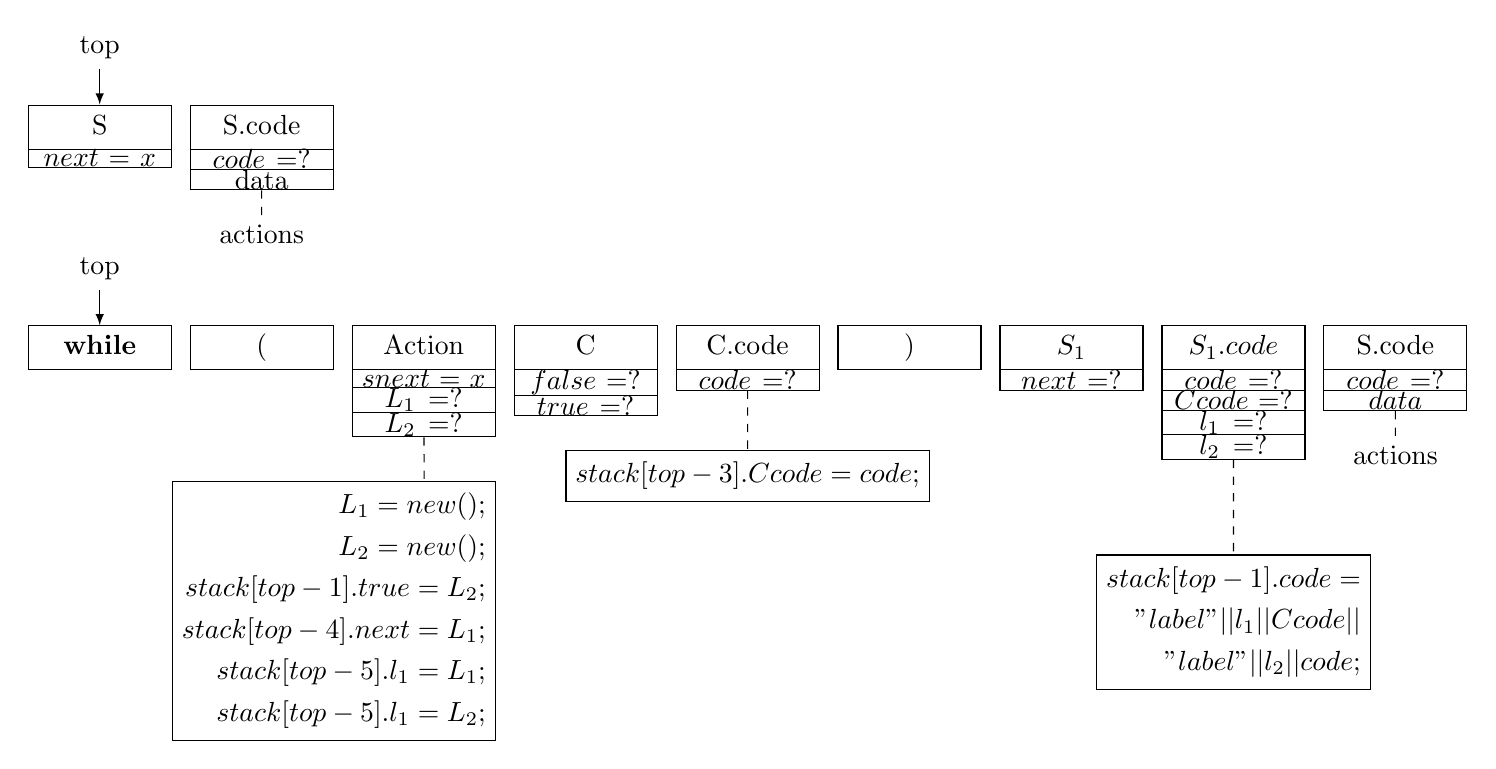
\begin{tikzpicture}[
  node distance = 1.5ex and 1.5ex,
  simple node/.style={
    draw,
    inner sep=0pt,
    minimum height = 3em,
    text width=12ex,
    text height=2.4ex,
    text depth=1.2ex,
    align=center,
    font=\linespread{.9}\selectfont,
  },
  split node/.style={
    simple node,
    rectangle split,
    rectangle split parts=#1,
    rectangle split ignore empty parts,
    rectangle split part align=base,
    draw,
    inner sep=0ex,
  },
  split horizon node/.style={
    simple node,
    rectangle split,
    rectangle split horizontal,
    rectangle split parts=#1,
    rectangle split ignore empty parts,
    draw,
    inner sep=0ex,
    rectangle split part align=base,
  },
  start chain=going mid right,
  every on chain/.append style={
  },
  ]
  {[start chain]
    \coordinate[on chain]  (9e6ea3d9-07fb-4e0d-84da-a93eeea20562)  at (0,0);
    \node[on chain,split node=2] (non-terminal) {S \nodepart{two} \(next=x\)};
    \node[on chain,split node=3] (s-syn) {S.code \nodepart{two}
      \(code=?\) \nodepart{three} data};
  }
  {[start chain]
    \node[on chain,split node=1,below=2 of non-terminal] (n1)
    {\textbf{while}};
    \node[on chain,split node=1] (n2)  {\((\)};
    \node[on chain,split node=4] (n3)  {Action \nodepart{two} \(snext=x\)
      \nodepart{three} \(L_{1}=?\) \nodepart{four} \(L_{2}=?\)};
    \node[on chain,split node=3] (n4)  {C \nodepart{two} \(false=?\)
      \nodepart{three} \(true=?\)};
    \node[on chain,split node=2] (n5) {C.code \nodepart{two} \(code=?\)};
    \node[on chain,split node=1] (n6)  {\()\)};
    \node[on chain,split node=2] (n7)  {\(S_{1}\) \nodepart{two} \(next=?\)};
    \node[on chain,split node=5] (n8) {\(S_{1}.code\)
      \nodepart{two} \(code=?\)
      \nodepart{three} \(Ccode=?\)
      \nodepart{four} \(l_{1}=?\)
      \nodepart{five} \(l_{2}=?\)
    };
    \node[on chain,split node=3] (n9) {S.code
      \nodepart{two} \(code=?\)
      \nodepart{three} \(data\)
    };
  }
  \node[below=0.32 of s-syn] (a0) {actions};

  \node[draw,below=0.55 of n3.south east,anchor=north east] (a1) {
    \(\begin{aligned}
        L_{1} = new();\\
        L_{2} = new();\\
        stack[top - 1].true = L_{2};\\
        stack[top - 4].next = L_{1};\\
        stack[top - 5].l_{1} = L_{1};\\
        stack[top - 5].l_{1} = L_{2};
      \end{aligned}\)
  };

  \node[draw,below=0.75 of n5] (a2) {
    \(\begin{aligned}
        stack[top - 3].Ccode = code;
      \end{aligned}\)
    };

    \node[draw,below=1.2 of n8] (a3) {
    \(\begin{aligned}
        stack[top - 1].code = \\
        "label" || l_{1} || Ccode || \\
        "label" || l_{2} || code;
      \end{aligned}\)
    };

    \node[below=0.32 of n9] (a4) {actions};

    \path (a1.north east) -- ++(-6ex,0) coordinate (a1p);
    \path[dashed,draw]
    (s-syn) -- (a0)
    (n3) -- (a1p)
    (n5) -- (a2)
    (n8) -- (a3)
    (n9) -- (a4);

    \node[above=0.45 of n1] (t2) {top};
    \node[above=0.45 of non-terminal] (t1) {top};

    \path[-latex,draw] (t1) -- (non-terminal);
    \path[-latex,draw] (t2) -- (n1);
\end{tikzpicture}
\end{document}
